\problem{The Scheming Gardener}

The Jackstraw Gardening Club is a cooperative of gardeners whose share
a common lot of land, parceling it out every year among their members,
each of whom gets their own plot of land within the larger lot.


Each winter, before the planting season, the club gathers together on
the lot to select their plots. Each member has a handful of wooden
stakes and a ball of string. Taking turns in rotation, each member may
choose to drive a new stake into the ground, and then may tie a length
of string between one or more pairs of stakes, forming a straight-line
connection between the two. Strings may not cross (except at the ends
where they are tied to same stake) nor may they lie directly atop one
another co-linearly. A string may not have both ends tied to the same
stake. Stakes may not be driven so close to an existing
string or stake that one could not easily step between them.

Each portion of the lot entirely surrounded by strings defines one
garden plot. The process continues until a majority of the club
members feel that enough enclosed plots have been formed, are willing
to stop, subject to the limitations:

\begin{itemize}

\item Upon stopping, any useless strings will be removed. A 
  useless string is one where the land just to each side of the string
  lies in the same plot or in the unenclosed portion of the lot.

\item At least one enclosed area must remain after removing the useless
  strings.

\item There will be no enclosed plots of zero area.

\item All the remaining strings (after the useless ones are removed)
  will be connected --- it will be possible to trace a path from one
  string to any other string in the lot.
\end{itemize}

The gardeners then choose their plots from among the enclosed areas.

\begin{wrapfigure}{r}{0.45\linewidth}
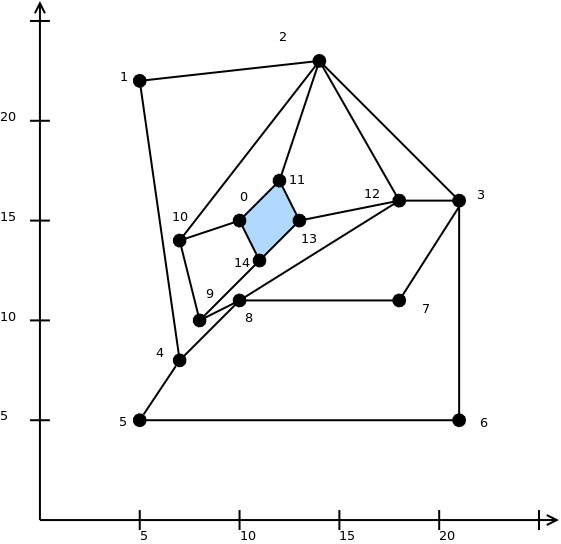
\includegraphics[width=\linewidth]{Gardener/plots1}
\end{wrapfigure}

You are lucky enough to have the first choice. You know that most of
your fellow gardeners will probably try for the largest area plots
they can get, but you have a different goal entirely. You are hoping
to raise a single, beautiful pumpkin that will win first prize at the
next county fair. You don't need much space, but you worry that your
pumpkins may be chewed upon by deer, rabbits, mice, and other
four-footed wildlife. You want to choose a plot that would force such
vermin to cross as many other plots as possible before reaching
yours. You hope that the sheer variety of crops presented by the other
gardeners will distract the vermin before they ever get to your plot. 
The vermin will not step directly on or over a stake, but will
always pass it to one side or the other.


\subsection*{Input}

Input will consist of 1 or more datasets.  Each dataset will begin
with a line containing two integers, $P$, and $E$. $2 < P \leq 750$, 
$3 \leq E \leq 1000$. A value of zero for $P$ indicates end of the input.

The first line of the dataset is followed by $P$ lines, each
containing $x,y$ coordinates of one point. These will be integers in the
range $0 \ldots \num{10000}$. These points will be distinct.

Those lines are followed by $E$ lines, each containing a pair of point
numbers, indicating a connection between those two points. These
numbers will be in the range $0\ldots P-1$ and refer to the order of
occurrence of the points in the earlier input, with point $0$ being the
first such point.


\subsection*{Output}

For each dataset, find a plot that maximizes the smallest number of
other plots that an animal approaching from outside would need to
cross before reaching your chosen one. Print the minimum number of
other plots that would need to be crossed by such an animal for your
chosen plot.


\subsection*{Example}


Here is a possible input:

\verbfile{Gardener/test0.in}


The output should be:

\verbfile{Gardener/test0.expected}


There are two datasets in the above input. The first, which ends with
the line containing ``0 14'', corresponds to the picture shown
above. The shaded plot in that picture is the one selected by the
scheming gardener.
